%!TEX root = ../main.tex

\section*{Results}

  \begin{figure}[h]
    \begin{center}
      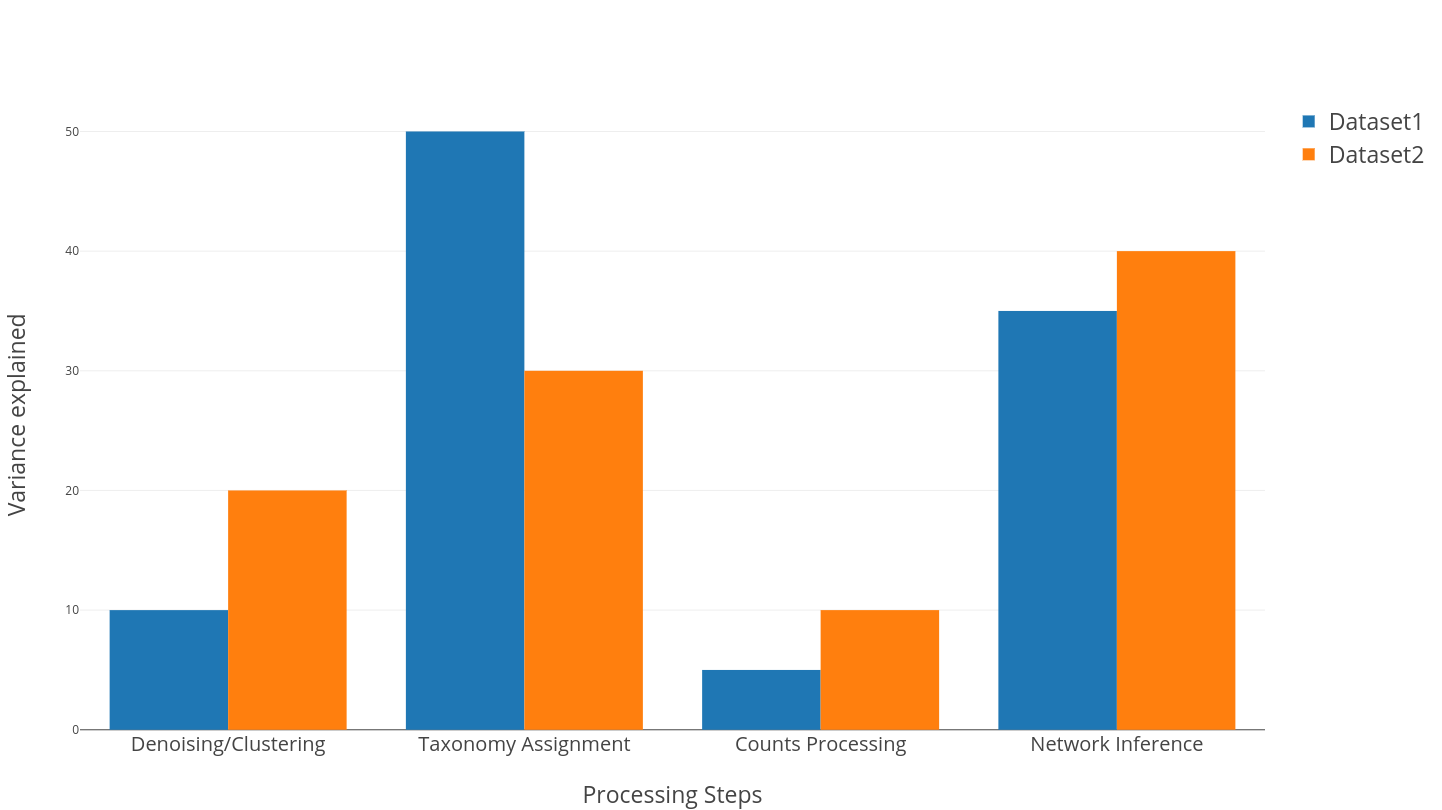
\includegraphics[width=17.8cm]{main_figure.png}
      \caption{\textbf{Percentage of variance in the final co-occurrence network due to each processing step.} }
      \label{fig:variance}
    \end{center}
  \end{figure}

  \begin{figure}[h]
    \begin{center}
      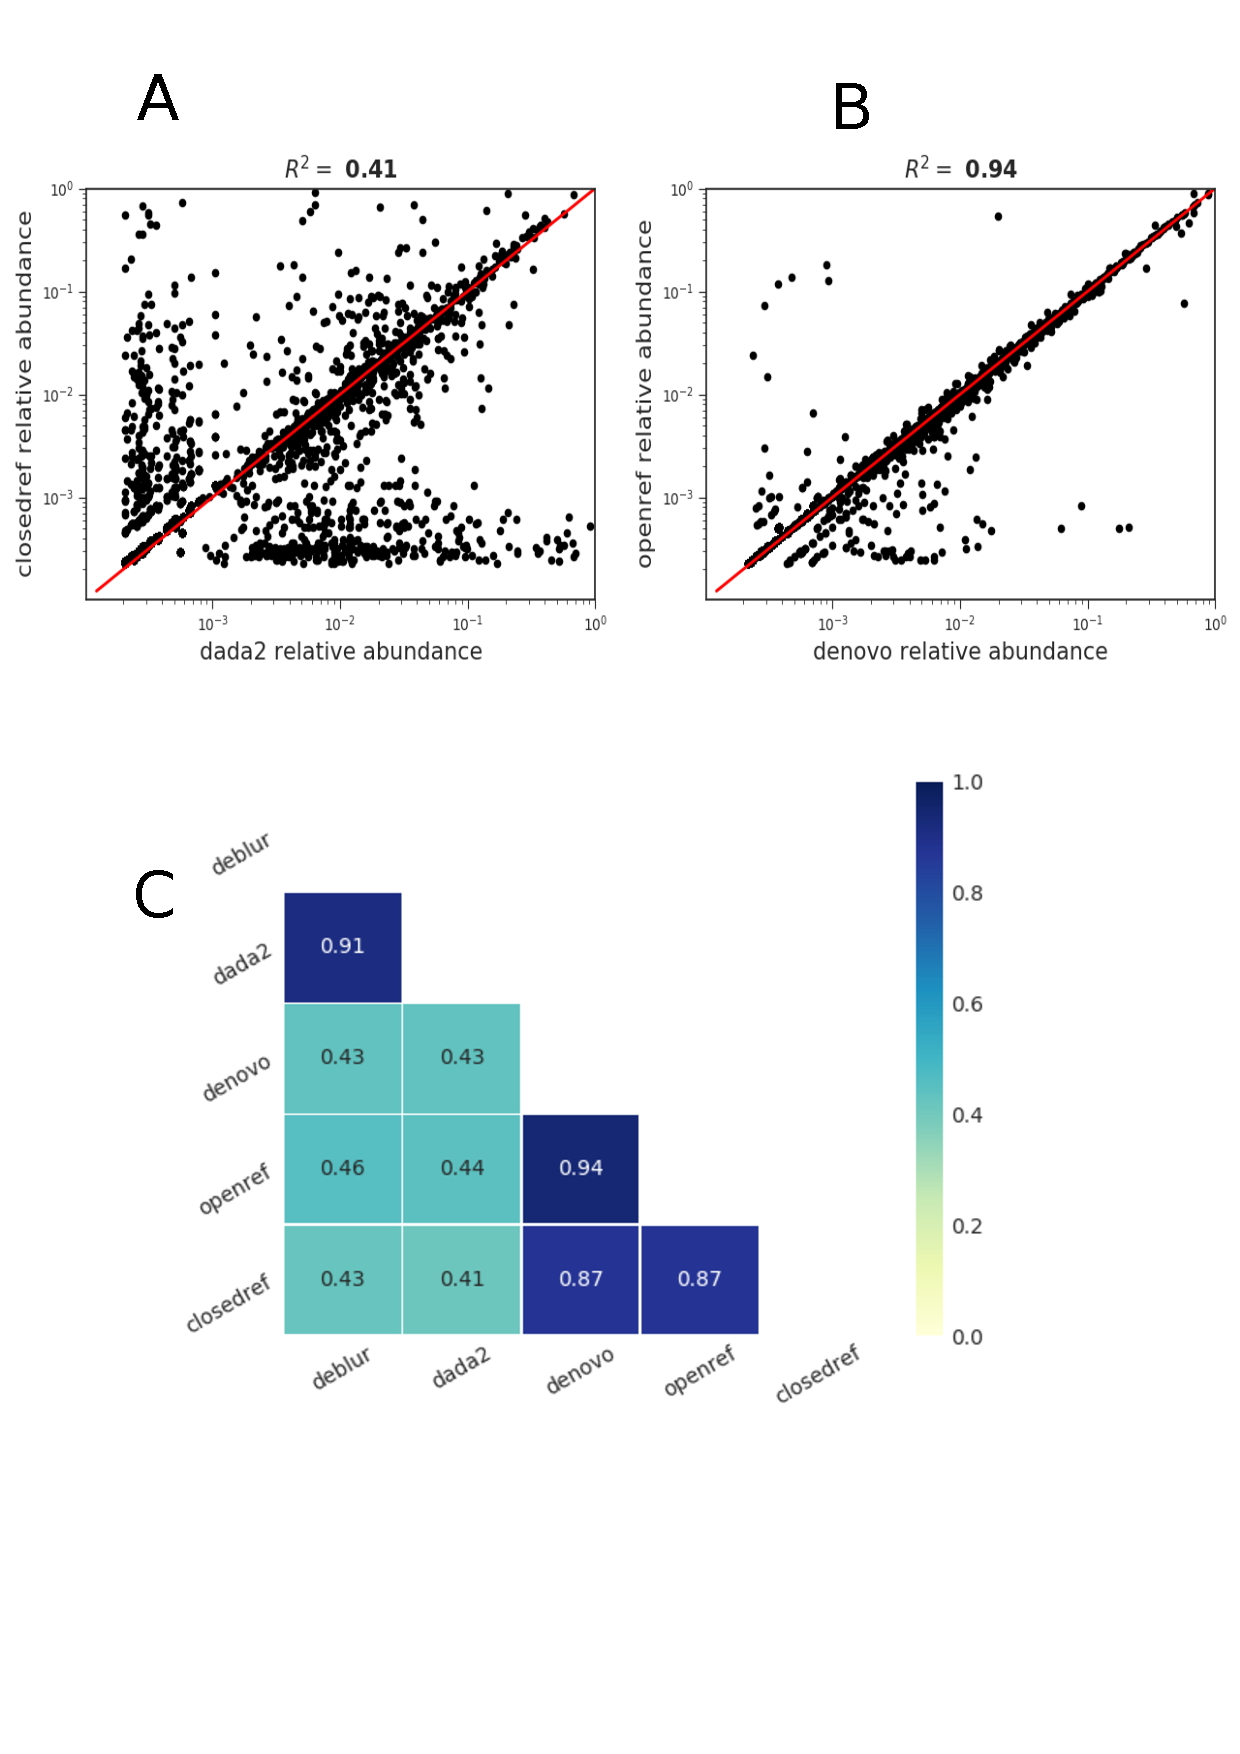
\includegraphics[width=15.8cm]{otu_corr_full.pdf}
      \caption{\textbf{Correlation between the abundances of taxa in OTU tables generated using various clustering and denoising methods}. }
      \label{fig:otu_correlations}
    \end{center}
  \end{figure}

  \begin{figure}[h]
    \begin{center}
      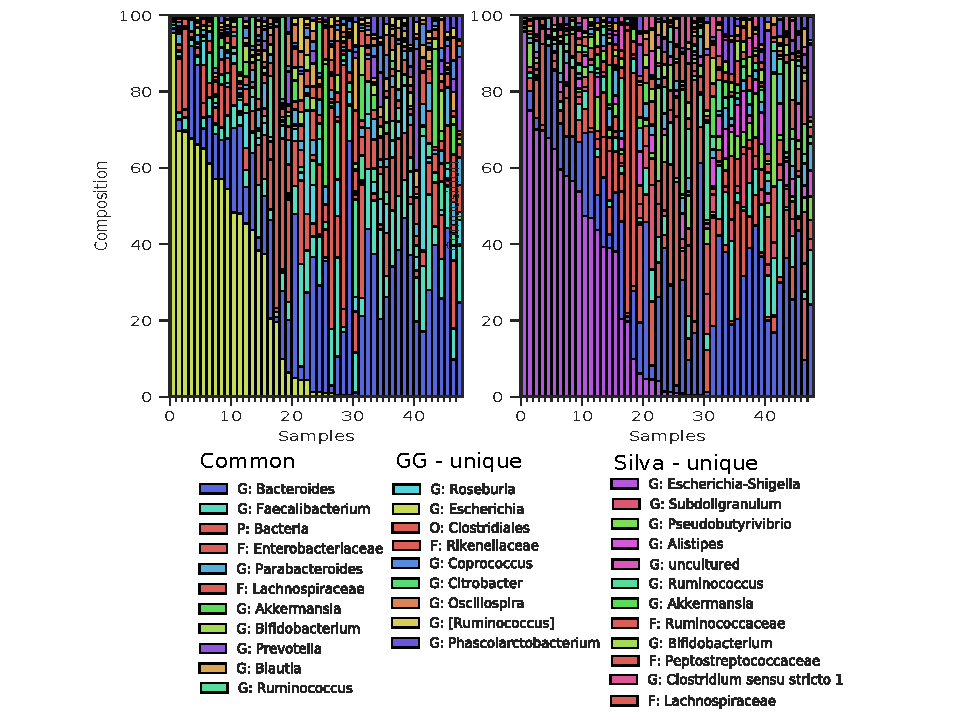
\includegraphics[width=17.8cm]{tax_comp_full.pdf}
      \caption{\textbf{Taxonomy composition of the 20 most abundant genera predicted using different taxonomy references databases}. NOTE: I will replace the legend with the taxonomy tree}
      \label{fig:tax_comp}
    \end{center}
  \end{figure}

  \begin{figure}[h]
    \begin{center}
      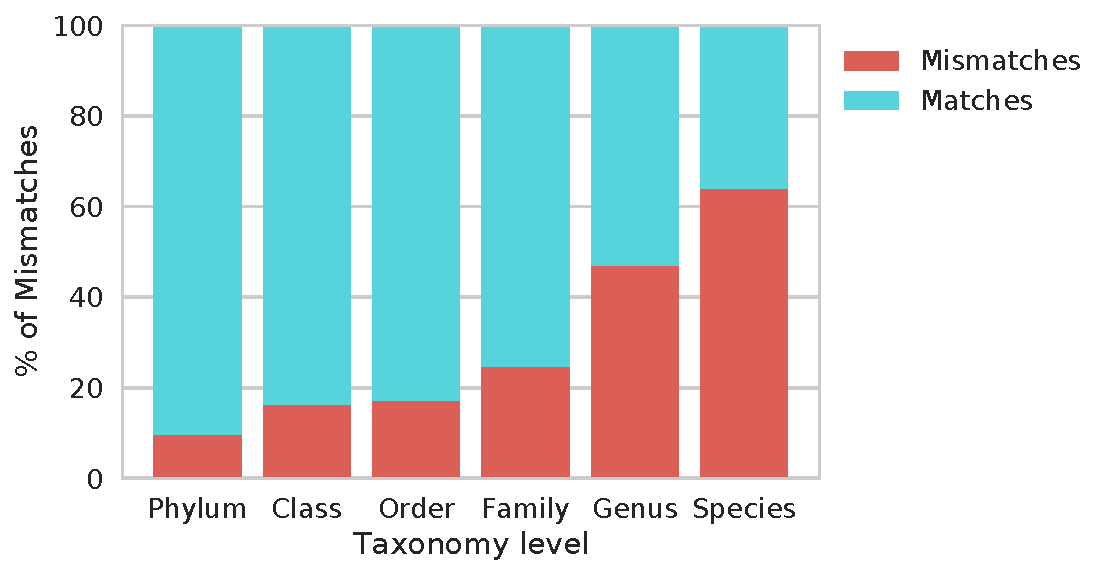
\includegraphics[width=15.8cm]{tax_distance_deblur.pdf}
      \caption{\textbf{Average percentage of mismatches in taxonomy assignment at various taxonomy levels}. NOTE: I will include a boxplot of the weighted distance in the taxonomy tree}
      \label{fig:otu_correlations}
    \end{center}
  \end{figure}

  \begin{figure}[h]
    \begin{center}
      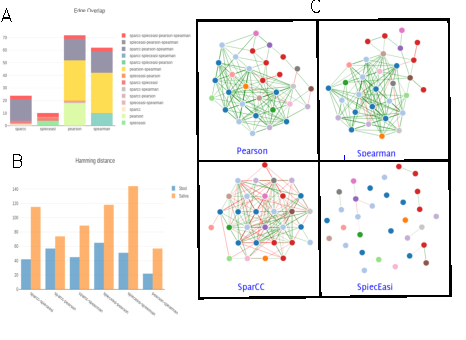
\includegraphics[width=17.8cm]{net_inference_comparison.pdf}
      \caption{\textbf{Variance of the co-occurrence networks for different processing pipelines}.  Node (\textbf{a})  and edge (\textbf{b}) overlap between all different networks generated from the data.}
      \label{fig:network_heatmap}
    \end{center}
  \end{figure}


  \begin{figure}[h]
    \begin{center}
      %\includegraphics[width=17.8cm]{../figures/network_comparison.pdf}
      \caption{\textbf{Core network captures known interactions in vaginal microbiota.} \textbf{a} Core network, obtained by taking the intersection between all the different pipelines. \textbf{b} Vaginal microbiota network as determined by XXX.}
      \label{fig:network_comparison}
    \end{center}
  \end{figure}


